\subsection{General Mapping Concept} \label{ssec:num2}

A semantic room map consists of four types of maps, an occupancy map, a object probability map, a room type map and a map with the locations of doorways. All those maps have to be consistent, which is difficult to achieve, as the environment is unknown and localization is uncertain. 

An elegant way to cope with the problem of uncertain localization causing inconsistencies between the maps is the usage of a simultaneous localization and mapping (SLAM) system based on a Rao-Blackwellized particle filter. Here the uncertainty of the robot pose is modeled using particles. Each particle creates its own map, which is done with mapping with known pose, as the pose of a particle has no uncertainty. Therefore additional maps containing other information are always consistent, as long as there is a separate map for every particle. When a map is requested the map attached to the currently most likely particle is returned. The major downside of this approach is that the computational cost increases with increasing number of particles, as every additional type of map has to be created for every particle separately. In our case, where every object type and every room type has its own map, the number of particles has to be very low.

Tests using GMapping, a 2D-SLAM library using Rao-Blackwellized particle filters and a sophisticated sampling technique, and a laser scanner showed good results, even with less than 10 particles. The use of GMapping splits the occupancy map into two parts, the 2D-SLAM and a 3D mapping with know pose for every particle. The 3D mapping is needed for the detection of obstacles not visible to the laser scanner and also in the object probability mapping, as can be seen later. The split of the metric mapping has another benefit. The crucial SLAM is done using only the accurate laser scanner while the comparable inaccurate depth image of the RGDB-camera is only used in the less important 3D mapping. The 3D mapping is done using the OctoMap, a 3D mapping framework based on Octrees.

The second fundamental concept is the hybrid map representation. Every room has its own semantic map. Each of these maps is a node in a topological map representing the room structure of the environment and an edge between two rooms states that the rooms are connected by a doorway. The edge further holds information about the corresponding mapped doorways in both rooms. Figure \ref{hybridmap} depicts a hybrid map example.

\begin{figure}[htp]
 \centering
 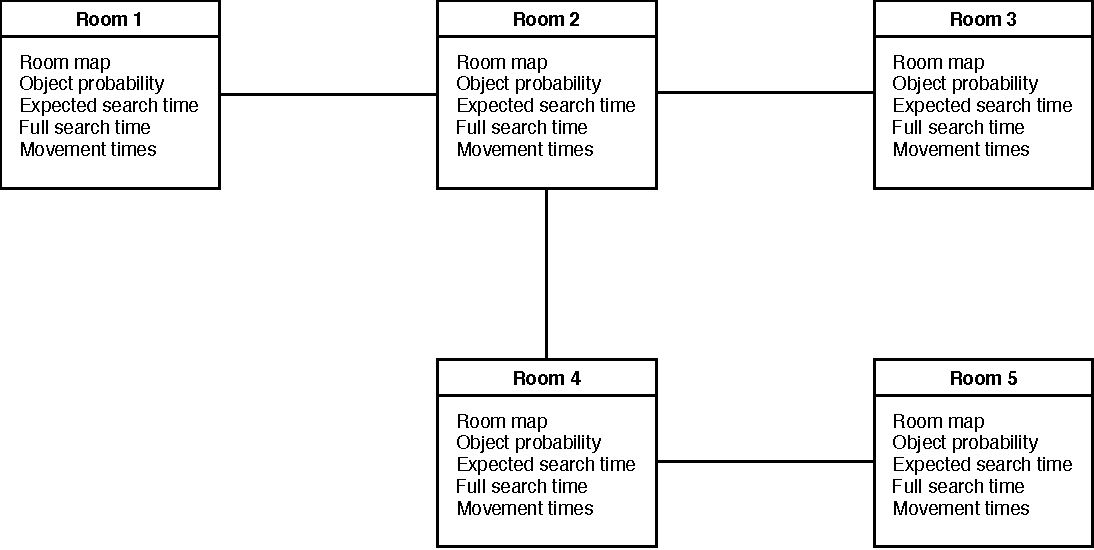
\includegraphics[width=1.\textwidth,trim={0 0 0 0},clip]{figures/HybridMap.pdf}
 \caption{hybrid map structure}
 \label{hybridmap}
\end{figure}


Every time a new doorway is found a new node is inserted into the topological map containing an empty room map. If a doorway is passed, the mapping in the old room is paused and the mapping in the new room is started (if it is the first time the robot enters this room) or resumed. When resuming, the poses of the doorway in both room coordinate frames are used to transform the robot position into the new rooms coordinate frame. Generally loops in the topological maps are possible, but no loop closure was implemented as there were no loops in the test environments.